アルゴリズムを実装し、各データセットにおけるアルゴリズムの実行時間をそれぞれ示す。実験環境は
\begin{description}
  \item[OS] Mac OS X El Caption (10.11.6)
  \item[CPU] Intel(R) Core(TM) i7-3770 CPU @ 3.40GHz
  \item[Memory] 16GB 1600MHz DDR3
\end{description}
でおこない、Algorithm \ref{MakeEpsilon}
\begin{algorithm}
  \caption{$\epsilon > 0$の与え方}
  \label{MakeEpsilon}
  \begin{algorithmic}
    \For {$i = 1$ to $10$}
      \For {$j = 9$ to $1$}
        \State $\epsilon = j \times 10^{-i}$
        \For {$k = 1$ to $100$}
          \State Main Procedureを$\epsilon$と実験で用いる$A_1, A_2, \cdots, A_m$を引数に呼び出し、実行時間を計測
        \EndFor
      \EndFor
    \EndFor
  \end{algorithmic}
\end{algorithm}
を使用してForループ1反復ごとの$\epsilon$とともにMain Procedureを100回呼び出してMain Procedureの実行時間から平均実行時間を算出した。実装はMATLAB 2016bを用いて行った。

\subsection{実験1}
\begin{align*}
  A_1 = \left(
            \begin{array}{ccc}
              2 &  0 &  0 \\
              0 &  0 & -1 \\
              0 & -1 &  0
            \end{array}
          \right),
  A_2 = \left(
            \begin{array}{ccc}
              0 & 0 & 0 \\
              0 & 1 & 0 \\
              0 & 0 & 0
            \end{array}
          \right),
  A_3 = \left(
            \begin{array}{ccc}
              0 & 0 & 1 \\
              0 & 0 & 0 \\
              1 & 0 & 0
            \end{array}
          \right),
  A_4 = \left(
            \begin{array}{ccc}
              0 & 1 & 0 \\
              1 & 0 & 0 \\
              0 & 0 & 0
            \end{array}
          \right)
\end{align*}
を問題として使用して実験を行った。この実験では双対問題\ref{DualSemidefiniteSystem}の許容解がアルゴリズムの結果として得られる。そのような例としては
\begin{align*}
    0 \cdot \left(
              \begin{array}{ccc}
                2 &  0 &  0 \\
                0 &  0 & -1 \\
                0 & -1 &  0
              \end{array}
            \right)
  + 2 \cdot \left(
              \begin{array}{ccc}
                0 & 0 & 0 \\
                0 & 1 & 0 \\
                0 & 0 & 0
              \end{array}
            \right)
  + 0 \cdot \left(
              \begin{array}{ccc}
                0 & 0 & 1 \\
                0 & 0 & 0 \\
                1 & 0 & 0
              \end{array}
            \right)
  + 0 \cdot \left(
              \begin{array}{ccc}
                0 & 1 & 0 \\
                1 & 0 & 0 \\
                0 & 0 & 0
              \end{array}
            \right)
\end{align*}
となる
\begin{align*}
  \mathbf{u} = \left(
                 \begin{array}{c}
                   0 \\
                   2 \\
                   0 \\
                   0
                 \end{array}
               \right)
\end{align*}
がある。実際、半正定値となるかを確認すると、
\begin{align*}
    0 \cdot \left(
              \begin{array}{ccc}
                2 &  0 &  0 \\
                0 &  0 & -1 \\
                0 & -1 &  0
              \end{array}
            \right)
  + 2 \cdot \left(
              \begin{array}{ccc}
                0 & 0 & 0 \\
                0 & 1 & 0 \\
                0 & 0 & 0
              \end{array}
            \right)
  + 0 \cdot \left(
              \begin{array}{ccc}
                0 & 0 & 1 \\
                0 & 0 & 0 \\
                1 & 0 & 0
              \end{array}
            \right)
  + 0 \cdot \left(
              \begin{array}{ccc}
                0 & 1 & 0 \\
                1 & 0 & 0 \\
                0 & 0 & 0
              \end{array}
            \right)
  = \left(
      \begin{array}{ccc}
        0 & 0 & 0 \\
        0 & 2 & 0 \\
        0 & 0 & 0
      \end{array}
    \right)
\end{align*}
の固有値は
\begin{align*}
  \det \left(\lambda I - \left(\begin{array}{ccc} 0 & 0 & 0 \\ 0 & 2 & 0 \\ 0 & 0 & 0\end{array}\right)\right) = x^2 \left(x - 2\right)
\end{align*}
から$\lambda = 2, 0$でどちらも非負となるので、この行列は半正定値である。

さて、この問題の下で作成したプログラムを実際に走らせると図\ref{test1}の実験結果が得られた。なお、横軸はMain Procedureに入力とする$\epsilon$を、縦軸は実行時間を表している。
\begin{figure}
  \centering
  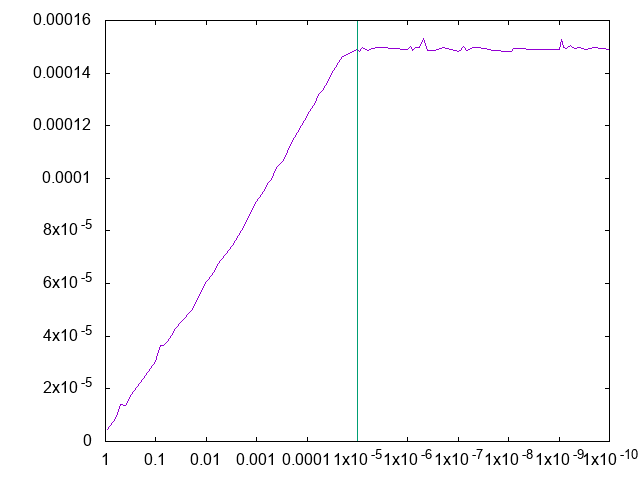
\includegraphics[width=10cm]{test1.png}
  \caption{実験1の実験結果}
  \label{test1}
\end{figure}

理論的には問題(\ref{MainSemidefiniteSystem})の許容解は出ずに、双対問題(\ref{DualSemidefiniteSystem})の許容解が結果として得られるはずであるが、$\epsilon$が大きい間はMain Procedureが先に終了してしまうため、アルゴリズムが解までたどり着くことができない。しかし、ある程度$\epsilon$が小さくなるとMain Procedureも十分な回数分反復することができるようになるため、理論的な結果と一致するようになったと考えられる。実際、図中の縦棒である、$10^{-5}$以降は理論的な結果と一致して双対問題(\ref{DualSemidefiniteSystem})の許容解が得られた。これ以降はどれほど$\epsilon$を小さくしようとも、双対問題(\ref{DualSemidefiniteSystem})の許容解が得られるため、実行時間が一定になっている。

\subsection{実験2}
\begin{align*}
  A_1 = \left(
            \begin{array}{ccc}
              0 &  0 &  0 \\
              0 &  1 & -1 \\
              0 & -1 &  0
            \end{array}
          \right),
  A_2 = \left(
            \begin{array}{ccc}
              0 & 0 & 0 \\
              0 & 1 & 0 \\
              0 & 0 & 0
            \end{array}
          \right),
  A_3 = \left(
            \begin{array}{ccc}
              0 &  0 &  0 \\
              0 & -1 &  0 \\
              0 &  0 & -2
            \end{array}
          \right) \\
\end{align*}
を問題として使用した。この実験では内点実行可能解が存在しないので、双対問題の解\ref{DualSolution}は存在することはなく、またどれほど$\epsilon$を小さくしても主問題(\ref{MainSemidefiniteSystem})の許容解を得ることはできない。

実際に実行して得られた結果は図\ref{test2}の通りである。なお、横軸はMain Procedureに入力とする$\epsilon$を、縦軸は実行時間を表している。
\begin{figure}
  \centering
  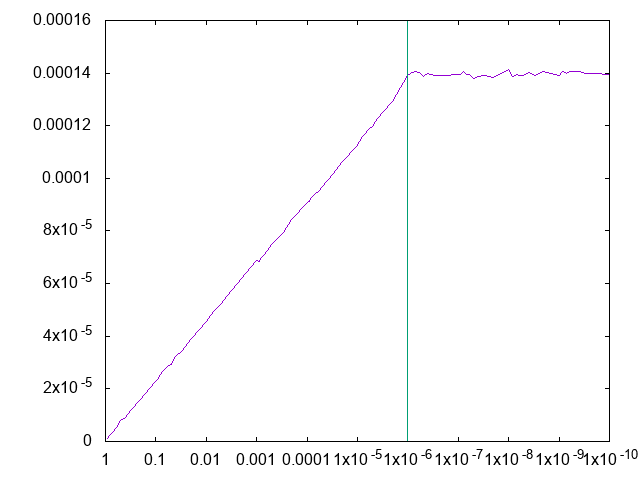
\includegraphics[width=10cm]{test2.png}
  \caption{実験2の実験結果}
  \label{test2}
\end{figure}
この結果から、アルゴリズムは内点実行可能解がない場合、$\epsilon$に依存して実行時間が伸びていることがわかる。

\subsection{実験3}
問題として使用する$A_1, A_2, \cdots, A_{30}$をMATLAB標準のrandnを用いて、Algorithm \ref{MakeRandomMatrices}のようにして生成を行った。この実験では乱数を用いたので、$A_1, A_2, \cdots A_{30}$を生成して、そしてそれらについて$\epsilon$ごとに30回実行時間を測定するということを1反復として実験を100回ほど行った。すなわち、$A_1, A_2, \cdots, A_{30}$に対してAlgorithm \ref{MakeEpsilon}を使用して、各$\epsilon$とともにMain Procedureの入力とし、$\epsilon$ごとに30回ほどその実行時間を測定した。
\begin{algorithm}
  \caption{$100$次実対称行列群$A_1, A_2, \cdots, A_{30}$の生成}
  \label{MakeRandomMatrices}
  \begin{algorithmic}
    \Input $\text{生成する整数の最小値} \And \text{生成する整数の最大値}$
    \For {$i = 1$ to $30$}
      \State $matrix \leftarrow \text{randn(100)}$
      \State $A_i \leftarrow matrix + matrix^T$
    \EndFor
  \end{algorithmic}
\end{algorithm}

実験結果は図\ref{randomtest}のようになった。なお、横軸はMain Procedureに入力とする$\epsilon$を、縦軸は実行時間を表している。
\begin{figure}
  \centering
  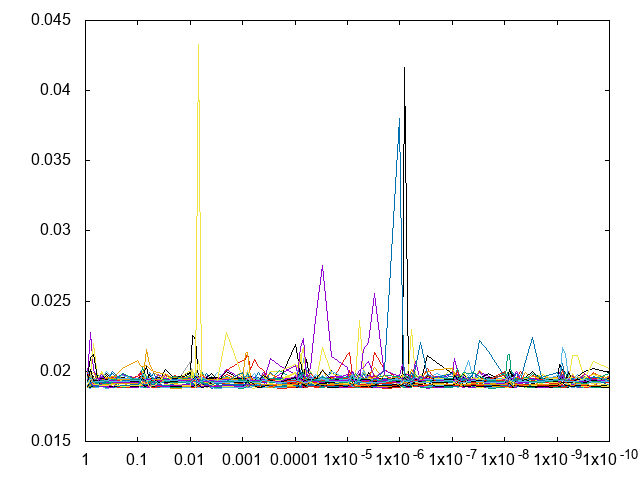
\includegraphics[width=10cm]{test3.png}
  \caption{実験3の実験結果}
  \label{randomtest}
\end{figure}

実験結果からExcelを用いて二元配置法を用いて、測定結果における分散分析表を作成した(表\ref{AnalysisOfVarianceTable})。なお有意水準$\alpha$は0.05と設定し、事前にShapiro-Wilk検定を用いて実行時間が繰り返しごとに正規分布に従うかを検定している(図\ref{Regular})。
\begin{figure}
  \centering
  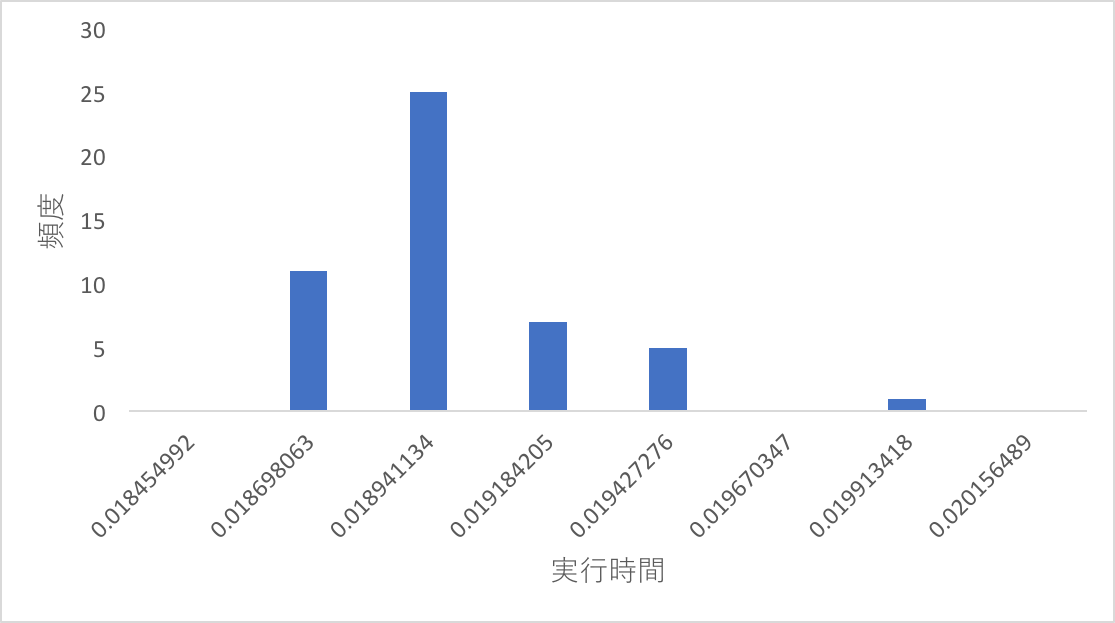
\includegraphics[width=10cm]{execute_time.png}
  \caption{もっとも最初に生成した問題の$\epsilon = 0.01$における実行時間の間隔のヒストグラム}
  \label{Regular}
\end{figure}
\begin{table}
  \centering
  \caption{実験3の分散分析表}
  \label{AnalysisOfVarianceTable}
  \begin{tabular}{c|cccccc} \hline
    要因         & 平方和     & 自由度   & 平均平方              & 分散比     & $p$値                 & $F$境界値 \\ \hline
    テスト       & $0.01444$ & $99$     & $0.0001458$            & $22.61$ & $0$ & $1.244736$ \\
    $\epsilon$   & $0.002241$  & $89$     & $3.5 \times 10^{-5}$  & $19.65009$ & $3.382 \times 10^{-32}$ & $1.2587$ \\
    交互作用     & $0.096$ & $8811$   & $1.098 \times 10^{-5}$ & $1.702$ & $0$                   & $1.025166$ \\
    繰り返し誤差 & $2.84512$ & $441000$ & $6.45 \times 10^{-6}$ &            &                       & \\ \hline
  \end{tabular}
\end{table}
すると、乱数で生成した問題と$\epsilon$において、$F$境界値よりも分散比の方が大きく、問題と$\epsilon$のどちらも実行時間に効果をもたらしていることがわかった。また、交互作用も$F$境界値の方が分散比よりも大きくなっており、作成した問題と$\epsilon$同士の組み合わせによる効果が実行時間に影響をもたらしていることも分かった。

この実験では$\epsilon$がどのような値であっても問題(\ref{MainSemidefiniteSystem})の許容解$X \succ 0$がみつかる。しかし、前述の実験のように$\epsilon$の値に応じて常に実行時間線形の値となるわけではなく、起伏が激しくなってしまった。これは実行時間が短かすぎたために、コンテキストスイッチなどのアルゴリズムとは本質的には関係ない実行時間による影響が大きくなってしまったのではないかと考えられる。

また、実行した際にえられた許容解の最小固有値を横軸に、縦軸を実行時間とすると、図\ref{eigen}のような結果が得られた。
\begin{figure}
  \centering
  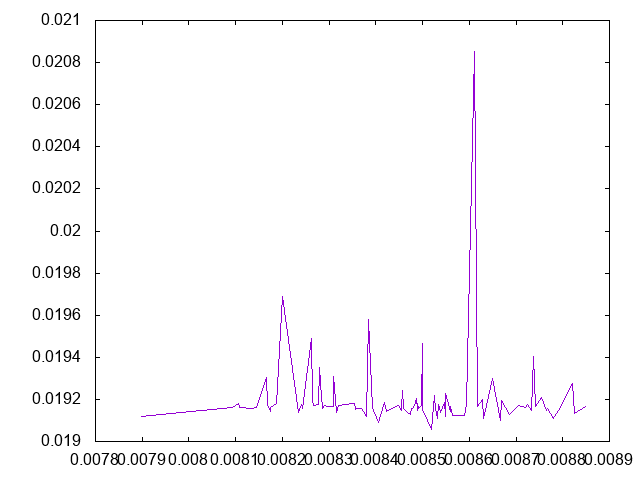
\includegraphics[width=10cm]{eigen.png}
  \caption{最小固有値と実行時間}
  \label{eigen}
\end{figure}
